\section{Distributed K Nearest Neighbor}

\vspace{5 mm}
\noindent
We would like to use a spill tree model on our data to categorize data with 
some likelihood of being close to our chosen data point. Once we 
construct the spill tree, classifying a point would then be as simple as 
performing a look up for the point (which would have complexity $O(P D)$ where 
$D = $ the depth of the spill tree) and then computing K Nearest Neighbor on 
the subset of the data, which if we set a threshold of the size of our child 
node equal to $U$ would be $O(U^{2} P)$ for a total time complexity of 
$O(P D + U^{2} P)$. Compared to our naive way of doing K Nearest Neighbor, 
this classification scheme with $U << N$, our runtime on classification is much 
less.

\vspace{5 mm}
\noindent
However, there are numerous problems when implementing a spill tree directly 
on our whole data set.

\begin{itemize}
\item Constructing our $D$ matrix in our spill tree algorithm is already  
$O(N^{2} P)$, so implementing a spill tree may help us for lookup, but will not 
help us in avoiding the time complexity of actually making the spill tree.
\item For data size large enough that it will not fit on a single machine, 
calculating a spill tree directly in a distributed environment will be 
near-impossible. Like K Nearest Neighbor, to construct a spill tree with 
perfect precision, we need to compare each data point to every other data 
point to determine the furthest two data points. On a distributed setting, this 
is impossible without a lot of computer communication.
\end{itemize}

\vspace{5 mm}
\noindent
Instead of constructing a spill tree on all of our data, we will instead 
implement an approximate hybrid spill tree. This approximation method will 
construct a sampled hybrid spill tree on one machine. This spill tree will 
classify our data into chunks of data that can fit on single machines. From 
there, we construct a spill tree on each of the distributed data sets[6].

\vspace{5 mm}
\noindent
The main problem with using a normal spill tree as our data structure is that if
$\tau$ is too large, the depth of the spill tree can go to infinity[6].  To prevent
this, we can use a hybrid spill tree.  Hybrid spill trees operate identically to
spill trees, except they have an additional parameter $\rho$, with $0 \le \rho <
1$  such that if the overlap proportion when $P.lc$ and $P.rc$ are constructed
is  $> \rho$, then $P.lc$ and $P.rc$ are instead simply split on the initial
bound with no overlap[6].  These nodes are marked as non-overlap, which will
become  important later on.  This guarantees that we will not have an infinite
depth  tree, and makes spill trees usable for our application.

\vspace{5 mm}
\noindent
We will be using a hybrid spill tree to store our data, because it will allow us
to make efficient approximate K nearest neighbor searches.  On a standard spill
tree with overlaps we would use defeatist search to implement K nearest
neighbors,  but it is important to remember that we now have non-overlap nodes
scattered  throughout, for which we would instead use the standard metric tree
depth first search.

\vspace{5 mm}
\noindent
This gives us an efficient data structure to use for our K nearest neighbors
algorithm, but it is still designed to be used in a serial environment, and we
want to use this in a distributed environment [6].  To accomplish this we will have
to somehow split the dataset among multiple machines.  This is problematic, as
to generate a hybrid spill tree, you need to have all of the data accessible in
memory.  We solve this by using the following procedure [6]:

\vspace{5 mm}
\noindent
\textbf{Distributed KNN - Algorithm}

\begin{itemize}
\item Sample our original data each with some probability.
\item Construct a spill tree using the algorithm in the previous section on the 
sampled data. We call this the top tree.
\item Classify all of our data according to the top tree. When we reach a 
leaf in the top tree, we will have a subset of the original data which we will 
send to a single machine on a distributed cluster.
\item On each distributed machine compute a spill tree on the subset of the 
data, again using the algorithm of the previous section. These are the bottom 
trees.
\item For each leaf of all the bottom trees, compute K nearest neighbor of the 
subset data. store the K closest points, classes, and distances.
\item If all of the data can fit on one machine, reduce the data to one 
machine. Duplicate data that went to more than one bottom tree will need to 
sort their list of values based on distances and return the K closest points.
\item If the data cannot fit on one machine, it us to the algorithm designer on 
how they wish to handle duplicate points. Data can be left distributed and 
accessed via top and bottom trees with duplicate data being compared upon data 
retrieval. We can mark duplicate data to be reduced to a machine to find the 
best update and then modify our top and bottom trees to send our classification 
down the correct path for the optimal closest points.
\end{itemize}

\newpage

\vspace{5 mm}
\noindent
We will provide an algorithm for when all of our data can fit on one machine:

\begin{algorithm}[ht!]
%-------------------------------Header------------------------------------------
\DontPrintSemicolon
\KwData{$X = N \times P + 1$ matrix of data, with each data $x_{i}$ having ID $i$.\\ 
\hspace{50pt} Have column $P + 1$ contain the class of $x_{i}$ \\
\hspace{29pt} $U = $ a specified threshold upper bound to stop splitting\\
\hspace{29pt} $\tau = $ our buffer parameter\\
\hspace{29pt} $D = N \times N $ matrix of all distances between $x_{i}$'s. \\
\hspace{50pt} Let $D[i, j] = $ distance between $x_{i}$ and $x_{j}$. \\
\hspace{29pt} $T_{acc} = $ our accumulated tree. Initialized to just a root node. \\
\hspace{29pt} $n_{curr} = $ a pointer to current node of $T_{acc}$ we are considering. \\
\hspace{29pt} $\frac{1}{M} = $ our sampling probability.}
\KwResult{$T = $ our spill tree}
%-------------------------------Body--------------------------------------------
\Begin{
    $S \leftarrow $ our sample dataset of $x_{i}$ sampled with probability $\frac{1}{M}$ \;
    $Top \leftarrow SpillTree(S)$ \;
    \textbf{MAPPER:} \;
    Label each leaf of $Top$ with a unique ID. \;
    Classify $X$ according to $Top$ \;
    For each $x_{i}$ in each child with ID $c_{id}$, emit ($c_{id}$, ($i$, $x_{i}$)) \;
    \textbf{REDUCER:} \;
    $Bottom \leftarrow SpillTree(X$ s.t. $c_{id}$'s are all equal$)$ \;
    For each leaf in $Bottom$ compute Naive K-NN \;
    emit ($i$, List[closest $K$ point ids, distances, and classes])
}
\caption{Distributed Spill Trees\label{DSP}}
\end{algorithm}

\vspace{5 mm}
\noindent
To assist, we have provided a flow chart to illustrate what we are doing. See 
figure 2.

\noindent\rule{12.1cm}{0.4pt}

\begin{figure}[ht!]
\centering
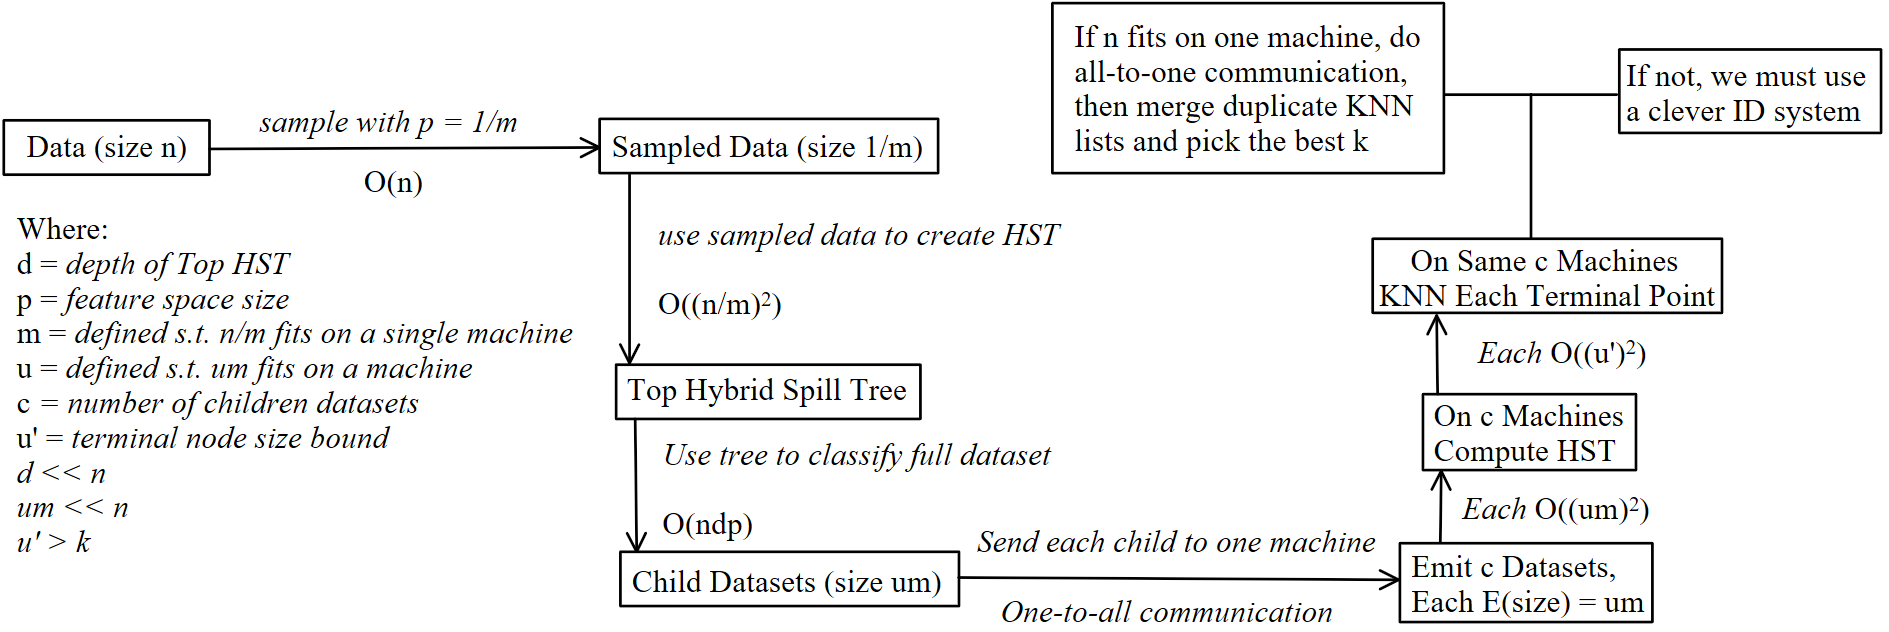
\includegraphics[width=0.9\textwidth]{algorithm}
\caption{A visualization of our algorithm to solve distributed K Nearest Neighbors}
\end{figure}

\noindent\rule{12.1cm}{0.4pt}

\vspace{5 mm}
\noindent
\textbf{Distributed KNN - Analysis}

\vspace{5 mm}
\noindent
This procedure works because the hybrid spill trees yield children subsets that,
with high probability, contain nodes that are close together [6].  This is true for 
hybrid spill trees more so than metric trees because in a metric tree, two points
that are very close together can be split into two different subtrees and never be
compared, but this does not happen in a hybrid spill tree [6].  In our algorithm, even
if two similar points happen to be separated in one of the children resulting from
a split, they will still be together in the other child, and so during evaluation 
it will still be considered.  This property can be seen below:

\vspace{5 mm}
\noindent\rule{12.1cm}{0.4pt}

\begin{figure}[ht!]
\centering
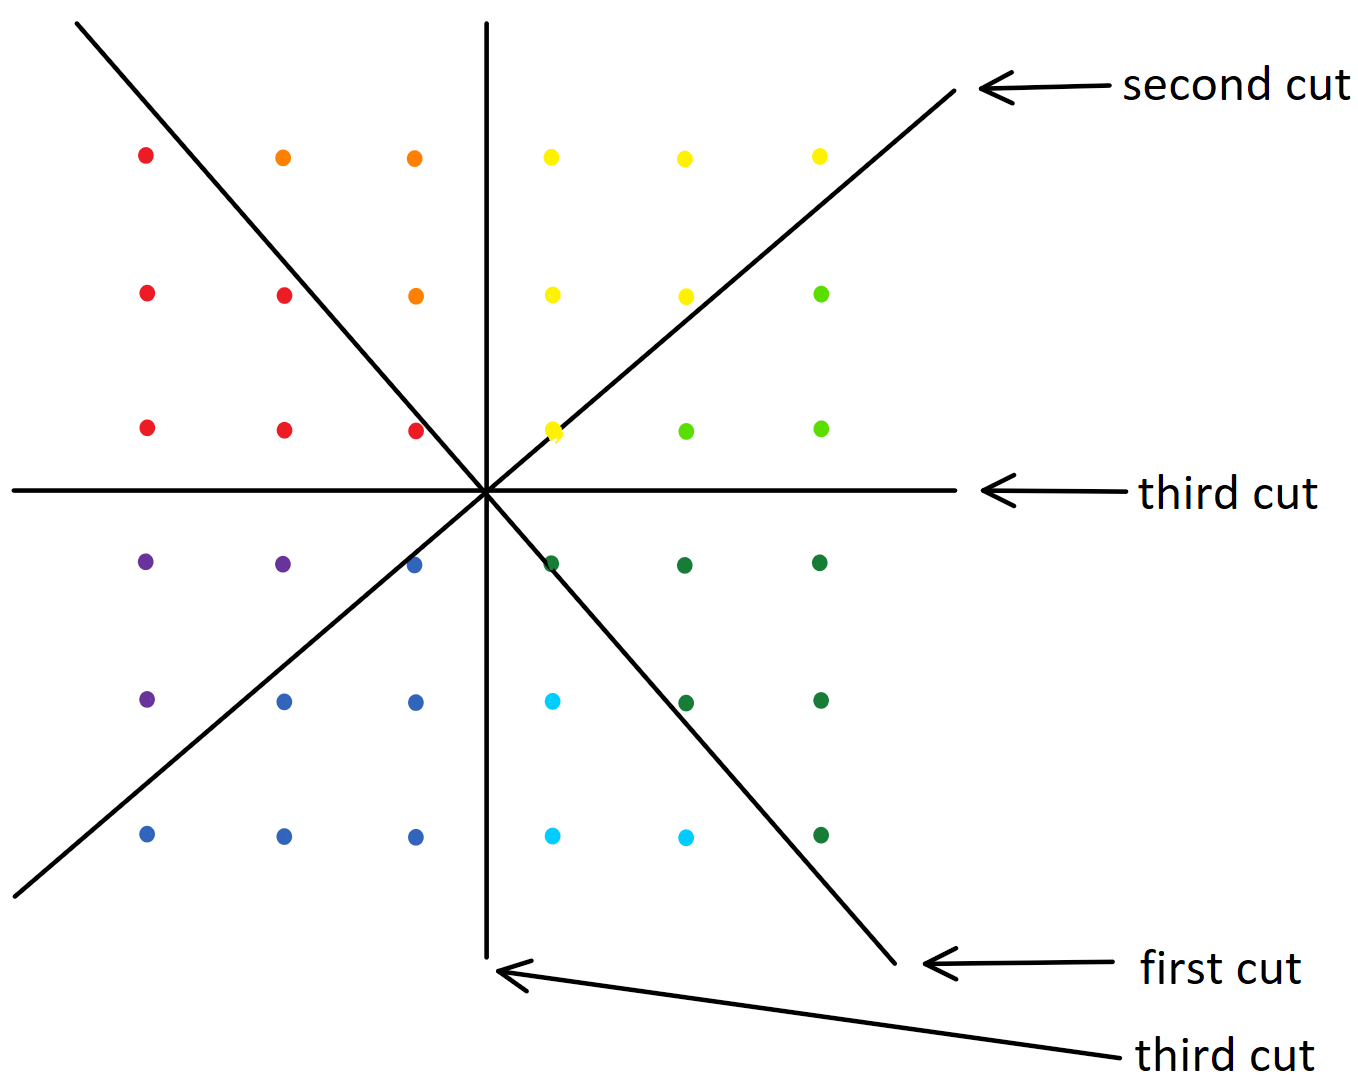
\includegraphics[width=0.9\textwidth]{metric}
\caption{In the metric tree, two points that are very close together will not 
be evaluated, whereas two points much further apart will be, because they 
happen to be in the same split}
\end{figure}

\noindent\rule{12.1cm}{0.4pt}

\newpage

\vspace{5 mm}
\noindent\rule{12.1cm}{0.4pt}

\begin{figure}[ht!]
\centering
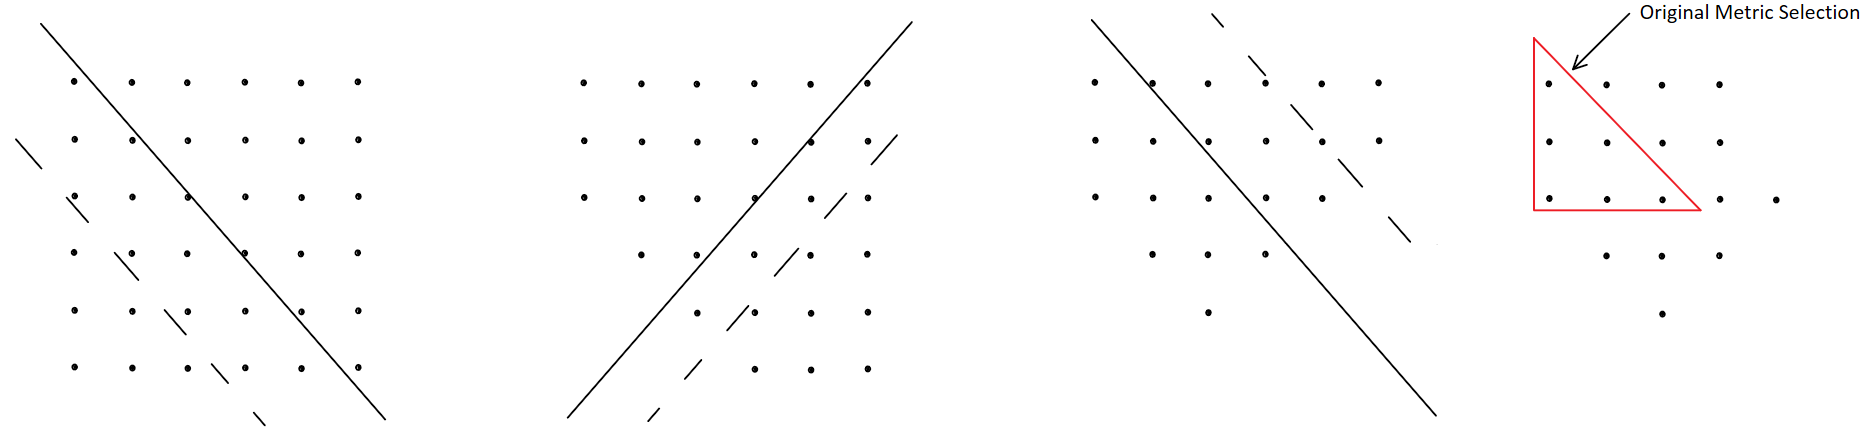
\includegraphics[width=0.9\textwidth]{spill}
\caption{In the spill tree, we can see that when comparing the corresponding
subset, there are much better odds of close together points being evaluated
together}
\end{figure}

\noindent\rule{12.1cm}{0.4pt}

\vspace{5 mm}
\noindent
In our algorithm we incur a one to all communication. We note that each leaf 
is of size $O(U M)$. Our total communication cost will be the sum of the size 
of each classified leaf. While we cannot guarantee that size given that that 
would depend on the construct of your data and the $\tau$ parameter we use, we 
know that it is at least of size $O(N)$. If we employ the use of the $\rho$ 
parameter to reduce duplications, we know that at most we will tollerate 
$\rho$ duplications per split. We can then bound our communication cost above 
by $N (1 + \rho)^{d}$. These are rough bounds - the real bounds heavily depend 
on the data set. Regardless, if your $N$ data cannot fit on a single machine, 
you would be hardpressed to compute K nearest neighbor without incurring a 
large amount of communication cost.

\vspace{5 mm}
\noindent
We also have an all to one communication towards the end where we send all of 
the K nearest neighbor lists to a machine, combining lists with identical keys. 
Without combining, the size of this cost will be equal to the initial 
communication cost because we have not gotten rid of any of our data at this 
point. When we combine, however, our data will again reduce down to size $N$.

\vspace{5 mm}
\noindent
We will now discuss the time complexity involved with computing:

\begin{itemize}
\item Sampling our data is $O(N)$ because we need to access every data element 
to sample. On an expected basis, the size of our sample will be $\frac{N}{M}$
\item Constucting our top tree strictly depends on how quickly we deplete our 
data when we perform a recurssive call. We know that outside the recurssive 
call we have $O(|S|^{2}) = O((\frac{N}{M})^{2})$ to perform regardless. On an 
expected basis.
\item Letting $D = $ the depth of the top tree, classifying all of our $N$ data 
will take $O(N P D)$ as argured earlier, because we will need to compare each 
data point against a boundary condition, which will be $O(P)$, and we will need 
to do that at most $D$ times for each of our $N$ data.
\item Once we have our data on each machine, each of expected size $U M$, we 
will need to compute another spill tree on each machine, again at least 
$O((U M )^{2})$.
\item Assuming we use the same threshold $U$ for our top and bottom tree, the 
leaves of each bottom tree will be size $O(U)$. Again, the number of leaves 
depends on our choice of $\tau$, $\rho$, and $U$, as well as our data shape. 
However, each leave will compute a naive K nearest neighbor, which is 
$O(P U^{2})$.
\end{itemize}

\vspace{5 mm}
\noindent
We notice from the above complexity analysis that the total time complexity 
requires us to know how many leaves we have in the top tree and the bottom 
trees. Our hope is that the number of leaves is such that our total time 
complexity is such that it is less than our naive $O(N^{2} P)$ method of 
computing K nearest neighbors. Regardless, if our data cannot fit on a single 
machine, we cannot hope to compute K nearest neighbor anyway without a 
distributed enviornment.

\vspace{5 mm}
\noindent
We notice that one of the advantages to our algorithm is that the runtime is heavily 
modifiable.  Some of our user parameters such as $M$ and $U$ are tuned according
to memory constraints or dataset size, but we can adjust $\tau$ and $\rho$ to 
bring down the runtime of our algorithm at the expense of accuracy, or increase 
the accuracy at the expense of the runtime [6].  Once you fit an initial model it is 
convenient to be able to optimize your accuracy, subject to your personal time 
constraints.  Consider our top tree, we know that when $\tau$ is 0 the model 
becomes metric, and that as $\tau$ increases the overlap will become greater and 
greater between pairs of children nodes.  It is therefore important to keep 
$\tau$ relatively low in the top tree, where a large amount of overlap will 
result in a greater compute time in the tope tree, as well as many more 
computations down the line when we are using our bottom trees [6].  In the bottom 
trees, however, it is less important to keep $\tau$ low, as multiple machines 
are making their spill tree computations in parallel, and we can afford to allow 
more overlap, as long as we set an appropriate value for $\rho$ to prevent the 
tree depth from getting out of hand.  Overall, the user defined parameters give 
our model a large degree of customization, and allow it to become optimized for 
the problem at hand.
